\documentclass[11pt, a4paper]{article}
\usepackage[english]{babel}
\usepackage[T1]{fontenc}
\usepackage[utf8x]{inputenc}
\usepackage{mathtools}
\usepackage{amsfonts}
\usepackage{array}
\usepackage{booktabs}
\usepackage{float}
\usepackage{algorithm}
\usepackage{algpseudocode}
\usepackage{hyperref}
\usepackage{tikz}
\usepackage{xcolor}
\usepackage{longtable}

\usetikzlibrary{trees}

\author{Francesco Landolfi \and Giorgio Vinciguerra}
\title{Exercises of Information Retrieval}

\newcommand{\exercise}{\subsection{Exercise} \paragraph{Question}}
\newcommand{\solution}{\paragraph{Solution}}
\newcommand{\hl}[1]{\colorbox{yellow}{#1}}

\begin{document}
\maketitle
% \clearpage
% --------------- DO NOT EDIT --------------- %
% This file has been automatically generated. %

\section{Crawling}
\exercise

Given a dictionary of $2^{16}$ strings,
%
\begin{itemize}

  \item compute the error rate of a Bloom Filter which uses an array of $2^{20}$
  bits and an optimal number of hash functions \emph{(assume that logs are in
  base 2)};

  \item say when the use of the Bloom Filter is advantageous in space with
  respect to the use of a standard hash table, given that the strings have
  length $L$ bits each and pointers cost 32 bits each.

\end{itemize}

\solution

The optimal number of hash functions is given by
%
\begin{align*}
  k = \frac{m}{n}\ln 2 = 2^4 \ln 2
\end{align*}
%
while the error rate is given by
%
\begin{align*}
  \varepsilon = \left( 1 - e^{-\frac{kn}{m}}\right)^k \approx 0.618^{16}.
\end{align*}

Regarding the second point, if we use an hash table then, only for the
initialization (\emph{without inserting any string in the dictionary}), for each
of its slot we have to allocate 2 pointers (one for the string, one for the
bucket), so $64 \cdot 2^d$ bits, where $d$ is the dimension of the dictionary.
For the Bloom Filter, instead, we have to allocate just $2^d$ bits, so the hash
table is alway disadvantageous.

\exercise

Assume that you have 7 items (6, 1, 3, 7, 2, 4, 9) and three servers whose IDs
are (1, 2, 3), and you want to distribute those items among the three servers
via consistent hashing. How would you do? What if a new server with ID 11 goes
up? \emph{(Hint: Instead of working on ring $[0,1]$, work on the integers in
$\{0,1, ... ,10\}$ using a universal hash function $h_a(x)= a*x \bmod m)$}

\solution

Given $a = 3$ we obtain that $h_3(1) = 3$, $h_3(2) = 6$, $h_3(3) = 9$. The items will be distributed as in the following table:
%
\begin{table}[h]
  \centering
  \begin{tabular}{l|c|c|c|c|c|c|c}
    item & 6 & 1 & 3 & 7 & 2 & 4 & 9 \\
    $h_3(\text{item})$ & 7 & 3 & 9 & 10 & 6 & 1 & 5 \\ \hline
    server ID & 3 & 1 & 3 & 1 & 2 & 1 & 2 \\
  \end{tabular}
\end{table}

If a new server with ID = 11 (and $h_3(11) = 0$) goes up, the item 7 will be
reassigned to that server.

\section{Locality-Sensitive Hashing}
\exercise

Given the binary vectors A = 10111, B = 10010, C = 00010, D = 00000 and E =
01100, apply LSH to find the similar vectors according to Hamming distance,
given $k = 2$ and $L = 2$. \emph{(Hint: use projections $I_1 = \{0, 3\}$, $I_2 =
\{3, 4\}$)}

\solution

First, we construct the sketch of each vector:
%
\begin{figure}[H]
  \hfill
  \begin{minipage}{0.45\columnwidth}
  \centering
  \begin{tabular}{c|c|c}
    {\bf v} & $I_1(\text{\bf v})$ & $I_2(\text{\bf v})$ \\ \hline
    A & 11 & 11 \\
    B & 11 & 10 \\
    C & 01 & 10 \\
    D & 00 & 00 \\
    E & 00 & 00 \\
  \end{tabular}
  \end{minipage}
  \begin{minipage}{0.45\columnwidth}
  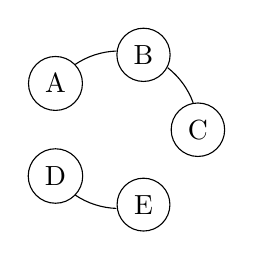
\begin{tikzpicture}
    \centering
    \def \radius {1cm}
    \def \margin {20}

    \node[draw, circle] at (0:\radius) {C};
    \draw[-, >=latex] ({0+\margin}:\radius)
      arc ({0+\margin}:{72-\margin}:\radius);
    \node[draw, circle] at (72:\radius) {B};
    \draw[-, >=latex] ({72+\margin}:\radius)
      arc ({72+\margin}:{144-\margin}:\radius);
    \node[draw, circle] at (144:\radius) {A};
    \node[draw, circle] at (216:\radius) {D};
    \draw[-, >=latex] ({216+\margin}:\radius)
      arc ({216+\margin}:{288-\margin}:\radius);
    \node[draw, circle] at (288:\radius) {E};

  \end{tikzpicture}
  \end{minipage}
  \hfill
\end{figure}
%
By the previous table, we can construct the similarity graph and conclude that:
%
\begin{itemize}
  \item A, B, C are similar;
  \item D, E are similar.
\end{itemize}

Alternatively, to speed up query time, we can construct an hash table for each
projection (each of size $2^{|I_i|}$) and use it as hash function, so to have:
%
\begin{table}[h]
  \centering
  \begin{tabular}{c|c|cc|c|c}
    \multicolumn{1}{c}{} &
    \multicolumn{1}{c}{$I_1$} &
    \multicolumn{1}{c}{} &
    \multicolumn{1}{c}{} &
    \multicolumn{1}{c}{$I_2$} & \\ \cline{2-2} \cline{5-5}
    00 & D, E & & 00 & D, E & \\ \cline{2-2} \cline{5-5}
    01 & C & & 01 & & \\ \cline{2-2} \cline{5-5}
    10 & & & 10 & B, C & \\ \cline{2-2} \cline{5-5}
    11 & A, B & & 11 & & \\ \cline{2-2} \cline{5-5}
  \end{tabular}
\end{table}

For example, given a new vector F = 11100, we compute the two projection,
$I_1(\text{F}) = 10$ and $I_2(\text{F}) = 00$, which point respectively to the
third and to the first cell of the two hash table, and find out that it is
similar to the vectors D and E. At this point we can compute explicitly the
Hamming distances:
%
\begin{align*}
  d(\text{F}, \text{D}) &= 3 \quad \text{\em (i.e., a false positive)},\\
  d(\text{F}, \text{E}) &= 1 \quad \text{\em (actually similar)}.
\end{align*}

\section{Documents Compression}
\exercise

Given the binary vectors A = 10111, B = 10010, C = 00010, D = 00000 and E =
01100, apply LSH to find the similar vectors according to Hamming distance,
given $k = 2$ and $L = 2$. \emph{(Hint: use projections $I_1 = \{0, 3\}$, $I_2 =
\{3, 4\}$)}

\solution

First, we construct the sketch of each vector:
%
\begin{figure}[H]
  \hfill
  \begin{minipage}{0.45\columnwidth}
  \centering
  \begin{tabular}{c|c|c}
    {\bf v} & $I_1(\text{\bf v})$ & $I_2(\text{\bf v})$ \\ \hline
    A & 11 & 11 \\
    B & 11 & 10 \\
    C & 01 & 10 \\
    D & 00 & 00 \\
    E & 00 & 00 \\
  \end{tabular}
  \end{minipage}
  \begin{minipage}{0.45\columnwidth}
  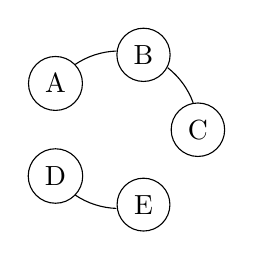
\begin{tikzpicture}
    \centering
    \def \radius {1cm}
    \def \margin {20}

    \node[draw, circle] at (0:\radius) {C};
    \draw[-, >=latex] ({0+\margin}:\radius)
      arc ({0+\margin}:{72-\margin}:\radius);
    \node[draw, circle] at (72:\radius) {B};
    \draw[-, >=latex] ({72+\margin}:\radius)
      arc ({72+\margin}:{144-\margin}:\radius);
    \node[draw, circle] at (144:\radius) {A};
    \node[draw, circle] at (216:\radius) {D};
    \draw[-, >=latex] ({216+\margin}:\radius)
      arc ({216+\margin}:{288-\margin}:\radius);
    \node[draw, circle] at (288:\radius) {E};

  \end{tikzpicture}
  \end{minipage}
  \hfill
\end{figure}
%
By the previous table, we can construct the similarity graph and conclude that:
%
\begin{itemize}
  \item A, B, C are similar;
  \item D, E are similar.
\end{itemize}

Alternatively, to speed up query time, we can construct an hash table for each
projection (each of size $2^{|I_i|}$) and use it as hash function, so to have:
%
\begin{table}[h]
  \centering
  \begin{tabular}{c|c|cc|c|c}
    \multicolumn{1}{c}{} &
    \multicolumn{1}{c}{$I_1$} &
    \multicolumn{1}{c}{} &
    \multicolumn{1}{c}{} &
    \multicolumn{1}{c}{$I_2$} & \\ \cline{2-2} \cline{5-5}
    00 & D, E & & 00 & D, E & \\ \cline{2-2} \cline{5-5}
    01 & C & & 01 & & \\ \cline{2-2} \cline{5-5}
    10 & & & 10 & B, C & \\ \cline{2-2} \cline{5-5}
    11 & A, B & & 11 & & \\ \cline{2-2} \cline{5-5}
  \end{tabular}
\end{table}

For example, given a new vector F = 11100, we compute the two projection,
$I_1(\text{F}) = 10$ and $I_2(\text{F}) = 00$, which point respectively to the
third and to the first cell of the two hash table, and find out that it is
similar to the vectors D and E. At this point we can compute explicitly the
Hamming distances:
%
\begin{align*}
  d(\text{F}, \text{D}) &= 3 \quad \text{\em (i.e., a false positive)},\\
  d(\text{F}, \text{E}) &= 1 \quad \text{\em (actually similar)}.
\end{align*}



\end{document}
